\documentclass{article}
\usepackage[utf8]{inputenc}
\usepackage[spanish,es-nodecimaldot,es-tabla]{babel}
\usepackage{amsmath}
\usepackage{graphicx}
\usepackage[colorlinks=true, allcolors=blue]{hyperref}
\usepackage[makeroom]{cancel}
% hyperref para autoref, amsmath para split
\usepackage{subfig,placeins}
\usepackage{libertine}
\usepackage[libertine]{newtxmath}
\graphicspath{{./figs/}{./imgs/}}
\usepackage[font=small,labelfont=bf]{caption}
\usepackage{listings,figs/tuneatantito}
\newcommand\pder[2]{\ensuremath {\dfrac{\partial#1}{\partial#2}}} 
\newcommand{\ppder}[2]{ \ensuremath {\dfrac{\partial^2 #1}{\partial #2^2}}}
\newcommand{\ppcder}[3]{ \ensuremath {\dfrac{\partial^2 #1}{\partial #2\partial #3}}}

\title{E1}
\author{{Pedraza-Espitia S.}}
\date{}

\begin{document}

\maketitle

\section{Ajuste}
\lstinputlisting[language=Matlab]{./MatlabCodes/E1_i4.m}
%%%%%
\begin{figure}[!hbt]
\centering
  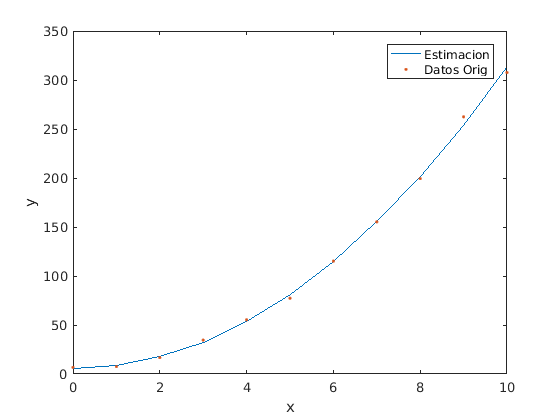
\includegraphics[width=0.6\textwidth]{E1_i4_ajuste}
	\caption{Ajuste por mínimos cuadrados.}%
	\label{fig:e1ajuste}
\end{figure}
%%%%%

\section{WRF, divergencia en  hurac\'an Ernesto}
\lstinputlisting[language=Matlab]{./MatlabCodes/E1_i5.m}
%%%%
\begin{figure}[!ht]
\centering
  \hfill\subfloat[Presión en superficie.]{
  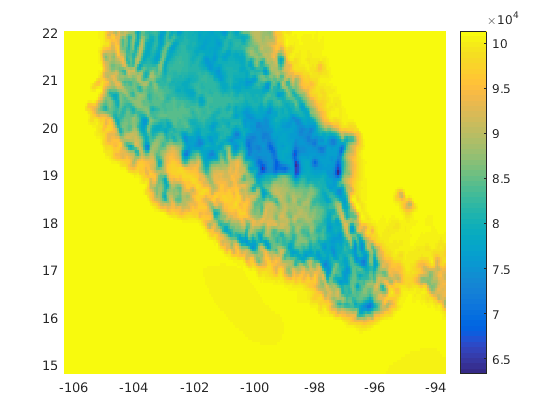
\includegraphics[width=0.35\textwidth]{E1_i5_a}
  }\hfill
  \subfloat[Divergencia.]{\label{sfig:div}
  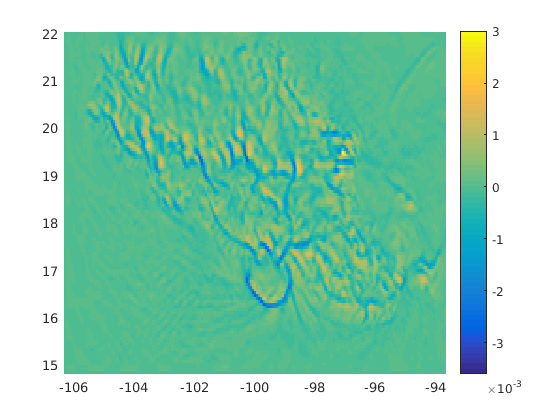
\includegraphics[width=0.35\textwidth]{E1_i5_c}
  }
\caption{(a) Gr\'afica de la presion de superficie. (b) Divergencia del viento en el tercer nivel; la divergencia es  máxima en long \mbox{-97.09}, lat 19.46; 10 de agosto/2012 a las 8:00 GMT.}%
\label{fig:netcdfdiver}
\end{figure}
%%%%%
%\FloatBarrier
\section{Runge-Kutta de orden 4}
\lstinputlisting[language=Matlab]{./MatlabCodes/E1_i6.m}
%%%%%
\begin{figure}[!hbt]
\centering
  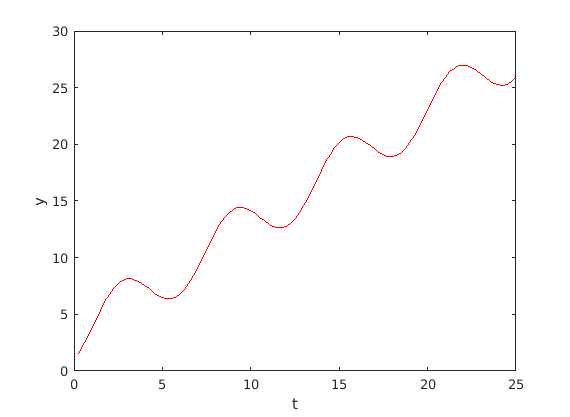
\includegraphics[width=0.6\textwidth]{E1_i6.png}
	\caption{Solución de $y'= 2\sin{t}+\cos{t}+1$.}%
	\label{fig:e1i6}
\end{figure}
%%%%%
\end{document}